\section{The case of small and medium dimension}\label{h1-sec}

In this section we establish lower bounds for $M_k$ (and related quantities, such as $M_{k,\eps}$) both for small values of $k$ (in particular, $k=3$ and $k=4$) and medium values of $k$ (in particular, $k=50$ and $k=54$).  Specifically, we will establish Theorem \ref{mlower}(vii), Theorem \ref{mke-lower}, and Theorem \ref{piece}.

\subsection{Bounding \texorpdfstring{$M_k$}{Mk} for medium \texorpdfstring{$k$}{k}}

We begin with the problem of lower bounding $M_k$.  We first formalize an observation\footnote{The arguments in \cite{maynard-new} are rigorous under the assumption of a positive eigenfunction as in Corollary \ref{ef}, but the existence of such an eigenfunction remains open for $k \geq 3$.} of Maynard \cite{maynard-new} that one may restrict without loss of generality to symmetric functions:

\begin{lemma}  For any $k \geq 2$, one has
$$ M_k \coloneqq \sup \frac{k J_1(F)}{I(F)}$$
where $F$ ranges over \emph{symmetric} square-integrable functions on ${\mathcal R}_k$ that are not identically zero.
\end{lemma}

\begin{proof}  Firstly, observe that if one replaces a square-integrable function $F: [0,+\infty)^k \to \R$ with its absolute value $|F|$, then $I(|F|) = I(F)$ and $J_i(|F|) \geq J_i(F)$.  Thus one may restrict the supremum in \eqref{mk4} to non-negative functions without loss of generality.  We may thus find a sequence $F_n$ of square-integrable non-negative functions on ${\mathcal R}_k$, normalized so that $I(F_n)=1$, and such that $\sum_{i=1}^k J_i(F_n) \to M_k$ as $n \to \infty$.

Now let 
$$\overline{F_n}(t_1,\dots,t_n) \coloneqq \frac{1}{n!} \sum_{\sigma \in S_n} F_n( t_{\sigma(1)},\dots,t_{\sigma(n)} )$$
be the symmetrization of $F_n$.  Since the $F_n$ are non-negative with $I(F_n)=1$, we see that
$$ I( \overline{F_n} ) \geq I( \frac{1}{n!} F_n ) = \frac{1}{(n!)^2}$$
and so $I(\overline{F_n})$ is bounded away from zero.  Also, from \eqref{mk4}, we know that the quadratic form
$$ Q(F) \coloneqq M_k I(F) - \sum_{i=1}^k J_i(F)$$
is positive semi-definite and is also invariant with respect to symmetries, and so from the triangle inequality for inner product spaces we conclude that
$$ Q( \overline{F_n} ) \leq Q( F_n ).$$
By construction, $Q(F_n)$ goes to zero as $n \to \infty$, and thus $Q(\overline{F_n})$ also goes to zero.  We conclude that 
$$ \frac{k J_1(\overline{F_n})}{I(\overline{F_n})} = \frac{\sum_{i=1}^k J_i(\overline{F_n})}{I(\overline{F_n})} \to M_k$$
as $n \to \infty$, and so
$$ M_k \geq \sup \frac{k J_1(F)}{I(F)}.$$
The reverse inequality is immediate from \eqref{mk4}, and the claim follows.
\end{proof}

To establish a lower bound of the form $M_k > C$ for some $C > 0$, one thus seeks to locate a symmetric function $F: [0,+\infty)^k \to \R$ supported on ${\mathcal R}_k$ such that
\begin{equation}\label{kjaf}
 k J_1(F) > C I(F).
\end{equation}
To do this numerically, we follow \cite{maynard-new} (see also \cite{gpy} for some related ideas) and can restrict attention to functions $F$ that are linear combinations
$$ F = \sum_{i=1}^n a_i b_i$$
of some explicit finite set $b_1,\dots,b_n: [0,+\infty)^k \to \R$ supported on ${\mathcal R}_k$, and some real scalars $a_1,\dots,a_n$ that we may optimize in.  The condition \eqref{kjaf} then may be rewritten as
\begin{equation}\label{ama}
 \mathbf{a}^T M_2 \mathbf{a} - C \mathbf{a}^T M_1 \mathbf{a} > 0
\end{equation}
where $\mathbf{a}$ is the vector 
$$ \mathbf{a} \coloneqq \begin{pmatrix} a_1 \\ \vdots \\ a_n \end{pmatrix}
$$
and $M_1,M_2$ are the real symmetric and positive semi-definite $n \times n$ matrices 
\begin{align*}
M_1 &= \left( \int_{\R^k} b_i(t_1,\dots,t_k) b_j(t_1,\dots,t_k)\ dt_1 \dots dt_k \right)_{1 \leq i,j \leq n} \\
M_2 &= \left( k \int_{\R^{k+1}} b_i(t_1,\dots,t_k) b_j(t_1,\dots,t_{k-1},t'_k)\ dt_1 \dots dt_k dt'_k\right)_{1 \leq i,j \leq n}.
\end{align*}
If the $b_1,\dots,b_n$ are linearly independent in $L^2({\mathcal R}_k)$, then $M_1$ is strictly positive definite, and (as observed in \cite[Lemma 7.3]{maynard-new}), one can find $\mathbf{a}$ obeying \eqref{ama} if and only if the largest eigenvalue of $M_2 M_1^{-1}$ exceeds $C$.  This is a criterion that can be numerically verified for medium-sized values of $n$, if the $b_1,\dots,b_n$ are chosen so that the matrix coefficients of $M_1,M_2$ are explicitly computable.

In order to facilitate computations, it is natural to work with bases $b_1,\dots,b_n$ of symmetric polynomials.  We have the following basic integration identity:

\begin{lemma}[Beta function identity]\label{bfi}  For any non-negative $a_1,\dots,a_k$, we have
$$ \int_{{\mathcal R}_k} t_1^{a_1} \dots t_k^{a_k}\ dt_1 \dots dt_k = \frac{\Gamma(a_1+1) \dots \Gamma(a_k+1)}{\Gamma(a_1+\dots+a_k+k+1)}$$
where $\Gamma(s) := \int_0^\infty t^{s-1} e^{-t}\ dt$ is the Gamma function.  In particular, if $a_1,\dots,a_k$ are natural numbers, then
$$ \int_{{\mathcal R}_k} t_1^{a_1} \dots t_k^{a_k}\ dt_1 \dots dt_k = \frac{a_1! \dots a_k!}{(a_1+\dots+a_k+k)!}.$$
\end{lemma}

\begin{proof}  If we write
$$ X := \int_{t_1+\dots+t_k=1} t_1^{a_1} \dots t_k^{a_k}\ dt_1 \dots dt_{k-1}$$
then by homogeneity we have
$$ r^{a_1+\dots+a_k+k-1} X = \int_{t_1+\dots+t_k=r} t_1^{a_1} \dots t_k^{a_k}\ dt_1 \dots dt_{k-1}$$
for any $r > 0$, and hence on integrating $r$ from $0$ to $1$ we conclude that
$$ \frac{X}{a_1+\dots+a_k+k} = \int_{{\mathcal R}_k} t_1^{a_1} \dots t_k^{a_k}\ dt_1 \dots dt_k.$$
On the other hand, if we multiply by $e^{-r}$ and integrate $r$ from $0$ to $\infty$, we obtain instead
$$ \int_0^\infty r^{a_1+\dots+a_k+k-1} X e^{-r}\ dr = \int_{[0,+\infty)^k} t_1^{a_1} \dots t_k^{a_k} e^{-t_1-\dots-t_k}\ dt_1 \dots dt_k.$$
Using the definition of the Gamma function, this becomes
$$ \Gamma(a_1+\dots+a_k+k) X = \Gamma(a_1+1) \dots \Gamma(a_k+1)$$
and the claim follows.
\end{proof}

Define a \emph{signature} to be a non-increasing sequence $\alpha = (\alpha_1,\alpha_2,\dots,\alpha_k)$ of natural numbers; for brevity we omit zeroes, thus for instance if $k=6$, then $(2,2,1,1,0,0)$ will be abbreviated as $(2,2,1,1)$.  The number of non-zero elements of $\alpha$ will be called the \emph{length} of the signature $\alpha$.  For each signature $\alpha$, we then define the symmetric polynomials $P_\alpha = P^{(k)}_\alpha$ by the formula
$$ 
P_\alpha(t_1,\dots,t_k) = \sum_{a: s(a)=\alpha} t_1^{a_1} \dots t_k^{a_k}$$
where the summation is over all tuples $a = (a_1,\dots,a_k)$ whose non-increasing rearrangement $s(a)$ is equal to $\alpha$.  Thus for instance
\begin{align*}
P_{(1)}(t_1,\dots,t_k) &= t_1 + \dots + t_k \\
P_{(2)}(t_1,\dots,t_k) &= t_1^2 + \dots + t_k^2 \\
P_{(1,1)}(t_1,\dots,t_k) &= \sum_{1 \leq i < j \leq k} t_i t_j \\
P_{(2,1)}(t_1,\dots,t_k) &= \sum_{1 \leq i < j \leq k} t_i^2 t_j + t_i t_j^2 
\end{align*}
and so forth.  Clearly, the $P_\alpha$ form a linear basis for the symmetric polynomials of $t_1,\dots,t_k$.  Observe that if $\alpha = (\alpha',1)$ is a signature containing $1$, then one can express $P_\alpha$ as $P_{(1)} P_{\alpha'}$ minus a linear combination of polynomials $P_\beta$ with the length of $\beta$ less than that of $\alpha$.  This implies that the functions $P_{(1)}^a P_\alpha$, with $a \geq 0$ and $\alpha$ avoiding the natural number $1$, are also a basis for the symmetric polynomials.  Equivalently, the functions $(1-P_{(1)})^a P_\alpha$ with $a \geq 0$ and $\alpha$ avoiding $1$ form a basis.

After extensive experimentation, we have discovered that a good basis $b_1,\dots,b_n$ to use for the above problem comes by setting the $b_i$ to be all the symmetric polynomials of the form $(1-P_{(1)})^a P_\alpha$, where $a \geq 0$ and $\alpha$ consists entirely of even numbers, whose total degree $a + \alpha_1+\dots +\alpha_k$ is less than or equal to some chosen threshold $d$.  For such functions, the coefficients of $M_1,M_2$ can be computed exactly using Lemma \ref{bfi}, as long as the degree $d$ is not too large {\bf give details}.

{\bf the text below is from a comment of Pace, needs to be edited in properly}

Fix some collection of symmetric polynomials $b_n\coloneqq b_n(x_1,\ldots, x_k)$.  (Ideally these polynomials are linearly independent.)  We then take $F=\sum_{n} c_n b_n$ for indeterminates $c_n$ which correspond to coordinates of the matrices after squaring.  In other words, the $(i,j)$ entry of $M_1$ is $\int_{\mathcal{R}_k} b_i b_j\ dx_1\ldots dx_k$.  So we need to find the types of monomials that occur in the product $b_i b_j$, and how often they occur in order to apply James' formula.  A similar computation is done for the $J$-integral although this is much slower, as the inner integral involves some expanding of terms.  This part of the computation is highly parallelizable and is not memory or CPU intensive; just time intensive.  [The computation is affected by the complexity of $\eps$, as we are doing exact arithmetic.  As will be clear a bit later, we could work with real approximations here if necessary.  This *might* speed things up, but I doubt it would be by much at present, and we would unfortunately lose our knowledge that the eventual output is a proven lower-bound.]

Currently this step takes a little more than half of the total time.  However, some of this time can be saved if one pre-computes a table of the monomials that occur in products $b_i b_j$ and $\left(\int_{0}^{1-\sum_{i=1}^{k-1}} b_i\ dx_k\right)\left(\int_{0}^{1-\sum_{i=1}^{k-1}} b_j\ dx_k\right)$.  This look-up table computation is also highly parallelizable, but at present is memory intensive.  If someone wants to work on finding a basis which (1) multiplies well, (2) integrates well with respect to the inner $J$-integral, and (3) from which it is easy to find which monomials occur, that would be very useful.  In particular, finding an algorithm to count the number and types of monomials in $e_1^{a_1}e_2^{a_2}\cdots e_k^{a_k}$ which is not memory intensive (and which is somewhat quick) would be very helpful.  [I imagine this is not a hard problem.  I just haven't thought about it yet.]

At present, the second step in the computation is to find the *exact* inverse of $M_1$.  This is the most memory intensive part of the program, and simply won't run in Mathematica without more than 64GB of RAM, when the degree gets to be about 20-22.  I'm currently playing with the other option that has been discussed recently, of instead just solving the generalized eigenvalue problem.  I don't know yet if this is less memory intensive (as implemented in Mathematica), but I believe it probably is.

The third step is to compute $M_3= M_1^{-1}M_2$ exactly.  This is relatively quick and easy.

Fourth, we compute a real approximation $M_3'$ to $M_3$.  This step is also very quick.  In the past we've been using 150 digit approximations in every entry, but I'm currently thinking this may have been extreme overkill (and may slow down subsequent steps).  We may be able to get by with many fewer digits (but not too many fewer, I'm still experimenting with this).

Fifth, we find an eigenvector $x'$ of $M_3'$, corresponding to the largest eigenvalue.  This step is not too long, nor too memory intensive; but I haven't been able to explore this step in the past because the computation of $M_1^{-1}$ was usually the hang-up.  We will likely replace this step with finding the generalized eigenvector. I expect the new computation to take about the same time as the old, but I don't have a lot of data yet.

Sixth, we find a rational approximation $x$ of the vector $x'$.  This is again very quick and easy.

Finally, we compute $(x^{T}M_2 x)/(x^{T}M_1 x)$ using exact arithmetic.  This is very quick, and the output is a proven lower bound on $M_{k,\eps}$.

If the generalized eigenvector functionality in Mathematica turns out to be less RAM intensive, then the new difficulty will be in building the look-up table for large degrees.


{\bf need to describe results of this method}



We now describe a second choice for the basis elements $b_1,\dots,b_n$, which uses the Krylov subspace method; it gives faster and more efficient numerical results than the previous basis, but does not seem to extend as well to more complicated variational problems such as $M_{k,\eps}$.  We introduce the linear operator ${\mathcal L}: L^2({\mathcal R}_k) \to L^2({\mathcal R}_k)$ defined by
$$ {\mathcal L} f( t_1,\dots,t_k) \coloneqq \sum_{i=1}^k \int_0^{1-t_1-\dots-t_{i-1}-t_{i+1}-\dots-t_k} f(t_1,\dots,t_{i-1},t'_i,t_{i+1},\dots,t_k)\ dt'_i.$$
This is a self-adjoint and positive semi-definite operator on $L^2({\mathcal R}_k)$.  For symmetric $b_1,\dots,b_n \in L^2({\mathcal R}_k)$, one can then write
\begin{align*}
M_1 &= \left( \langle b_i, b_j \rangle \right)_{1 \leq i,j \leq n} \\
M_2 &= \left( \langle {\mathcal L} b_i, b_j \rangle \right)_{1 \leq i,j \leq n}.
\end{align*}
If we then choose
$$ b_i \coloneqq {\mathcal L}^{i-1} 1$$
where $1$ is the unit constant function on ${\mathcal R}_k$, then the matrices $M_1,M_2$ take the Toeplitz form
\begin{align*}
M_1 &= \left( \langle {\mathcal L}^{i+j-2} 1, 1 \rangle \right)_{1 \leq i,j \leq n} \\
M_2 &= \left( \langle {\mathcal L}^{i+j-1} 1, 1 \rangle \right)_{1 \leq i,j \leq n},
\end{align*}
and so can be computed entirely in terms of the $2n$ numbers $\langle {\mathcal L}^i 1, 1 \rangle$ for $i=0,\dots,2n-1$.  

The operator ${\mathcal L}$ maps symmetric polynomials to symmetric polynomials; for instance, one has
\begin{align*}
{\mathcal L} 1 &= k - P_{(1)} \\
{\mathcal L} P_{(1)} &= \frac{k}{2} - \frac{k-1}{2} P_{(2)} - (k-2) P_{(1,1)}
\end{align*}
and so forth.  From this and Lemma \ref{bfi}, the quantities $\langle {\mathcal L}^i 1, 1 \rangle$ are explicitly computable rational numbers; for instance, one can calculate
\begin{align*}
\langle 1, 1 \rangle &= \frac{1}{k!} \\
\langle {\mathcal L} 1, 1\rangle &= \frac{2k}{(k+1)!} \\
\langle {\mathcal L}^2 1, 1\rangle &= \frac{k (5k+1)}{(k+2)!} \\
\langle {\mathcal L}^3 1, 1\rangle &= \frac{2k^2 (7k+5)}{(k+3)!} 
\end{align*}
and so forth.



...

\subsection{Bounding \texorpdfstring{$M_{k,\eps}$}{Mk,epsilon} for medium \texorpdfstring{$k$}{k}}

...

{\bf describe the modifications needed to the first $M_k$ method that can handle $M_{k,\eps}$}

\subsection{Bounding \texorpdfstring{$M_{4,0.18}$}{M4,0.18}}

We now prove Theorem \ref{mke-lower}(xii'), which can be established by a direct numerical calculation.  We introduce the explicit function $F: [0,+\infty)^4 \to \R$ defined by 
$$ F(t_1,t_2,t_3,t_4) \coloneqq (1 - \alpha (t_1+t_2+t_3+t_4)) 1_{t_1+t_2+t_3+t_4 \leq 1+\eps}$$
with $\eps \coloneqq 0.18$ and $\alpha \coloneqq 0.784$.  As $F$ is symmetric in $t_1,t_2,t_3,t_4$, we have $J_{i,1-\eps}(F) = J_{1,1-\eps}(F)$, so to show Theorem \ref{mke-lower}(xii') it will suffice to show that
\begin{equation}\label{jf}
 \frac{4 J_{1,1-\eps}(F)}{I(F)} > 2.00444.
\end{equation}
By making the change of variables $s=t_1+t_2+t_3+t_4$ we see that
\begin{align*}
I(F) &= \int_{t_1+t_2+t_3+t_4 \leq 1+\eps} (1-\alpha(t_1+t_2+t_3+t_4))^2\ dt_1 dt_2 dt_3 dt_4 \\
&= \int_0^{1+\eps} (1-\alpha s)^2 \frac{s^3}{3!}\ ds\\
&= \alpha^2 \frac{(1+\eps)^6}{36} - \alpha \frac{(1+\eps)^5}{15} + \frac{(1+\eps)^4}{24} \\
&= 0.0073005\dots
\end{align*}
and similarly by making the change of variables $u = t_1+t_2+t_3$
\begin{align*}
J_{1,1-\eps}(F) &= \int_{t_1+t_2+t_3 \leq 1-\eps} (\int_0^{1+\eps-t_1-t_2-t_3} (1-\alpha(t_1+t_2+t_3+t_4))\ dt_4)^2 dt_1 dt_2 dt_3 \\
&= \int_0^{1-\eps} (\int_0^{1+\eps-u} (1-\alpha(u+t_4))\ dt_4)^2 \frac{u^2}{2!} du \\
&= \int_0^{1-\eps} (1+\eps-u)^2 (1-\alpha \frac{1+\eps+u}{2})^2 \frac{u^2}{2} du  \\
&= 0.00365836\dots
\end{align*}
and so \eqref{jf} follows.

\begin{remark}  If we use the truncated function
$$ \tilde F(t_1,t_2,t_3,t_4) \coloneqq F(t_1,t_2,t_3,t_4) 1_{t_1,t_2,t_3,t_4 \leq 1}$$
in place of $F$, one can compute that
$$ \frac{4 J_{1,1-\eps}(\tilde F)}{I(\tilde F)} > 2.00235.$$
Thus it is possible to establish Theorem \ref{mke-lower}(xii') using a cutoff function $F'$ that is also supported in the unit cube $[0,1]^4$.  This allows for a slight simplification to the proof of $\DHL[4,2]$ assuming GEH, as one can add the additional hypothesis $S(F_{i_0})+S(G_{i_0}) < 1$ to Theorem \ref{nonprime-asym}(ii) in that case.
\end{remark}

\begin{remark} By optimising in $\eps$ and taking $F$ to be a symmetric polynomial of degree higher than $1$, one can get slightly better lower bounds for $M_{4,\eps}$; for instance setting $\eps = 5/21$ and choosing $F$ to be a cubic polynomial, we were able to obtain the bound $M_{4,\eps} \geq 2.05411$.  On the other hand, the best lower bound for $M_{3,\eps}$ that we were able to obtain was $1.91726$ (taking $\eps = 56/113$ and optimizing over cubic polynomials).  {\bf maybe a link to the code etc. is warranted here.}
\end{remark}

\subsection{Three-dimensional cutoffs}\label{3d}

In this section we establish Theorem \ref{piece}.  We relabel the variables $(t_1,t_2,t_3)$ as $(x,y,z)$, thus our task is to locate a piecewise polynomial function 
$F: [0,+\infty)^3 \to \R$ supported the simplex
$$ R := \{ (x,y,z) \in [0,+\infty)^3: x+y+z \leq \frac{3}{2}$$
and symmetric in the $x,y,z$ variables, obeying the vanishing marginal condition
\begin{equation}\label{fmor}
\int_0^\infty F(x,y,z)\ dz = 0
\end{equation}
whenever $x,y \geq 0$ with $x+y > 1+\eps$, and such that
\begin{equation}\label{tt1}
J(F) > 2 I(F)
\end{equation}
where
\begin{equation}\label{jf-def}
J(F) := 3\int_{x+y \leq 1-\eps} (\int_0^\infty F(x,y,z)\ dz)^2\ dx dy
\end{equation}
and
\begin{equation}\label{if-def}
I(F) := \int_R  F(x,y,z)^2\ dx dy dz
\end{equation}
and
$$\eps := 1/4.$$

Our strategy will be as follows.  We will decompose the simplex $R$ (up to null sets) into a carefully selected set of disjoint open polyhedra $P_1,\dots,P_m$ (in fact $m$ will be $60$), and on each $P_i$ we will take $F(x,y,z)$ to be a low degree polynomial $F_i(x,y,z)$ (indeed, the degree will never exceed $5$).  The left and right-hand sides of \eqref{tt1} become quadratic functions in the coefficients of the $F_i$.  Meanwhile, the requirement of symmetry, as well as the marginal requirement \eqref{fmor}, imposes some linear constraints on these coefficients.  In principle, this creates a finite-dimensional quadratic program, which one can try to solve numerically.  However, to make this strategy practical, one needs to keep the number of linear constraints imposed on the coefficients to be fairly small, as compared with the total number of coefficients.  To achieve this, the following properties on the polynomials $P_i$ are desirable:

\begin{itemize}
\item (Symmetry) If $P_i$ is a polytope in the partition, then every reflection of $P_i$ formed by permuting the $x,y,z$ coordinates should also lie in the partition.
\item (Graph structure) Each polytope $P_i$ should be of the form 
\begin{equation}\label{qi-form}
\{ (x,y,z): z \in Q_i; a_i(x,y) < z < b_i(x,y)\},
\end{equation}
where $a_i(x,y), b_i(x,y)$ are linear forms and $Q_i$ is a polygon.
\item (Epsilon splitting)  Each $Q_i$ is contained in one of the regions $\{ (x,y): x+y < 1-\eps\}$, $\{ (x,y): 1-\eps < x+y < 1+\eps \}$, or $\{ (x,y): 1+\eps < x+y < 3/2 \}$.
\end{itemize}

Observe that the vanishing marginal condition \eqref{fmor} now takes the form
\begin{equation}\label{vanish}
 \sum_{i: (x,y) \in Q_i} \int_{a_i(x,y)}^{b_i(x,y)} F_i(x,y,z)\ dz = 0
\end{equation}
for every $x,y > 0$ with $x+y > 1+\eps$.  If the set $\{i: (x,y) \in Q_i\}$ is fixed, then the left-hand side of \eqref{vanish} is a polynomial in $x,y$ whose coefficients depend linearly on the coefficients on the $F_i$, and thus \eqref{vanish} imposes a set of linear conditions on these coefficients for each possible set $\{ i: (x,y) \in Q_i\}$ with $x+y > 1+\eps$.

Now we describe the partition we will use.  This partition can in fact be used for all $\eps$ in the interval $[1/4,1/3]$, but the endpoint $\eps = 1/4$ has some simplifications and appears to be the optimal choice of this parameter.  To obtain the symmetry axiom, it is natural to split $R$ (modulo null sets) into six polyhedra $R_{xyz}, R_{xzy}, R_{yxz}, R_{yzx}, R_{zxy}, R_{zyx}$, where
$$ R_{xyz} := \{(x,y,z)\in R\ :\ x+y < y+z < z+x\} = \{(x,y,z): 0 < y < x < z; x+y+z \leq 3/2 \}$$
and the other polyhedra are obtained by permuting the indices $x,y,z$, thus for instance
$$ R_{yxz} := \{(x,y,z)\in R\ :\ y+x < x+z < z+y\} = \{(x,y,z): 0 < x < y < z; x+y+z \leq 3/2 \}.$$
%The polytope $R_{xyz}$ is a tetrahedron with vertices $(0,0,0), (0,0,3/2), (3/4,0,3/4), (1/2,1/2,1/2)$, and similarly for the other five polyhedra.

To obtain the epsilon splitting axiom, we decompose $R_{xyz}$ (modulo null sets) into eight sub-polytopes
\begin{align*}
A_{xyz} & =\{(x,y,z)\in R\ :\ x+y< y+z< z+x< 1-\eps\},\\
B_{xyz} & =\{(x,y,z)\in R\ :\ x+y< y+z< 1-\eps< z+x< 1+\eps\},\\
C_{xyz} & =\{(x,y,z)\in R\ :\ x+y< 1-\eps < y+z < z+x< 1+\eps\},\\
D_{xyz} & =\{(x,y,z)\in R\ :\ 1-\eps < x+y<  y+z < z+x< 1+\eps\},\\
E_{xyz} & =\{(x,y,z)\in R\ :\ x+y< y+z< 1-\eps <  1+\eps < z+x\},\\
F_{xyz} & =\{(x,y,z)\in R\ :\ x+y< 1-\eps < y+z <  1+\eps < z+x\},\\
G_{xyz} & =\{(x,y,z)\in R\ :\ x+y< 1-\eps  <  1+\eps < y+z < z+x\},\\
H_{xyz} & =\{(x,y,z)\in R\ :\ 1-\eps < x+y<  y+z < 1+\eps < z+x\};
\end{align*}
the other five polytopes $R_{xyz}, R_{yxz}, R_{yxz}, R_{zxy}, R_{zyx}$ are decomposed similarly, leading to a partition of $R$ into $6 \times 8 = 48$ polytopes.
This is almost the partition we will use; however there is a technical difficulty arising from the fact that some of the permutations of $F_{xyz}$ do not obey the graph structure axiom.  So we will split $F_{xyz}$ further, into the three pieces
\begin{align*}
S_{xyz} & = \{(x,y,z)\in F_{xyz}\ :\ z< 1/2+\eps\},\\
T_{xyz} & = \{(x,y,z)\in F_{xyz}\ :\ z> 1/2+\eps;x> 1/2-\eps \}, \\
U_{xyz} & = \{(x,y,z)\in F_{xyz}\ :\ x< 1/2-\eps \}.
\end{align*}
Thus $R_{xyz}$ is now partitioned into ten polytopes $A_{xyz}, B_{xyz}, C_{xyz}, D_{xyz}, E_{xyz}, S_{xyz}, T_{xyz}, U_{xyz}, G_{xyz}, H_{xyz}$, and similarly for permutations of $R_{xyz}$, leading to a decomposition of $R$ into $6 \times 10 = 60$ polytopes.

%Geometrically, $A_{xyz}$ is a tetrahedron with vertices $(0,0,0), (0,0,1-\eps), (1/2-\eps/2,0,1/2-\eps/2), (1/2-\eps/2,1/2-\eps/2,1/2-\eps/2)$; $B_{xyz}$ is a polytope with vertices $(1/2-\eps/2,0,1/2-\eps/2)$, $(1/2-\eps/2,1/2-\eps/2,1/2-\eps/2)$, $(1/2+\eps/2,0,1/2+\eps/2)$, $(1/2+\eps/2,1/2-3\eps/2,1/2+\eps/2)$, $(0,0,1-\eps)$, $(2\eps,0,1-\eps)$; ...

A symmetric piecewise polynomial function $F$ supported on $R$ can now be described (up to almost everywhere by specifying a polynomial function $F\downharpoonright_{P}: P \to \C$ for the ten polytopes $P = A_{xyz}, B_{xyz}, C_{xyz}, D_{xyz}, E_{xyz},  S_{xyz}, T_{xyz}, U_{xyz}, G_{xyz}, H_{xyz}$, and then extending by symmetry, thus for instance
$$ F\downharpoonright_{A_{yzx}}(x,y,z) = F\downharpoonright_{A_{xyz}}(z,x,y).$$

As discussed earlier, the expressions $I(F), J(F)$ can now be written as quadratic forms in the coefficients of the $F\downharpoonright_P$, and the vanishing marginal condition \eqref{fmor} imposes some linear constraints on these coefficients.

Observe that the polytope $D_{xyz}$ and all of its permutations make no contribution to either the functional $J(F)$ or to the marginal condition \eqref{fmor}, and give a non-negative contribution to $I(F)$.  Thus without loss of generality we may assume that
$$ F\downharpoonright_{D_{xyz}} = 0.$$
However, the other nine polytopes $A_{xyz}, B_{xyz}, C_{xyz}, E_{xyz}, S_{xyz}, T_{xyz}, U_{xyz}, G_{xyz}, H_{xyz}$ have at least one permutation which gives a non-trivial contribution to either $J(F)$ or to \eqref{fmor}, and cannot be easily eliminated.

Now we compute $I(F)$.  By symmetry we have
$$ I(F) = 3! I(F \downharpoonright_{R_{xyz}} ) = 6 \sum_P I( F \downharpoonright_P ) $$
where $P$ ranges over the nine polytopes $A_{xyz}, B_{xyz}, C_{xyz}, E_{xyz}, S_{xyz}, T_{xyz}, U_{xyz}, G_{xyz}, H_{xyz}$.  A tedious but straightforward computation shows that
\begin{align*}
I(F\downharpoonright_{A_{xyz}}) & =\int_{x=0}^{1/2-\eps/2}\int_{y=0}^{x}\int_{z=x}^{1-\eps-x}F\downharpoonright_{A_{xyz}}^2\ dz\ dy\ dx \\
I(F\downharpoonright_{B_{xyz}}) &= \left(\int_{z=1/2-\eps/2}^{1/2+\eps/2}\int_{x=1-\eps-z}^{z} +\int_{z=1/2+\eps/2}^{1-\eps}\int_{x=1-\eps-z}^{1+\eps-z}\right) \int_{y=0}^{1-\eps-z}F\downharpoonright_{B_{xyz}}^2\ dy\ dx\ dz \\
I(F\downharpoonright_{C_{xyz}}) & = \left(\int_{y=0}^{1/2-3\eps/2} \int_{x=y}^{y+2\eps} + \int_{y=1/2-3\eps/2}^{1/2-\eps}\int_{x=y}^{1-\eps-y} \right) \int_{z=1-\eps-y}^{1+\eps-x} \\ & + \int_{y=1/2-\eps}^{1/2-\eps/2}\int_{x=y}^{1-\eps-y}\int_{z=1-\eps-y}^{3/2-x-y} F\downharpoonright_{C_{xyz}}^2\ dz\ dx\ dy \\
I(F\downharpoonright_{E_{xyz}}) & = \int_{z=1/2+\eps/2}^{1-\eps}\int_{x=1+\eps-z}^{z}\int_{y=0}^{1-\eps-z} F\downharpoonright_{E_{xyz}}^2\ dy\ dx\ dz \\
I(F\downharpoonright_{S_{xyz}}) & =  \left(\int_{y=0}^{1/2-3\eps/2}\int_{z=1-\eps-y}^{1/2+\eps} +\int_{y=1/2-3\eps/2}^{1/2-\eps}\int_{z=y+2\eps}^{1/2+\eps} \right)\int_{x=1+\eps-z}^{1-\eps-y} F\downharpoonright_{S_{xyz}}\ dx\ dz\ dy \\
I(F\downharpoonright_{T_{xyz}}) &  = \left(\int_{z=1/2+\eps}^{1/2+2\eps}\int_{x=1+\eps-z}^{3/2-z} + \int_{z=1/2+2\eps}^{1+\eps}\int_{x=1/2-\eps}^{3/2-z}\right)\int_{y=0}^{3/2-x-z} F\downharpoonright_{T_{xyz}}^2\ dy\ dz\ dx \\
I(F\downharpoonright_{U_{xyz}}) & = \int_{x=0}^{1/2-\eps}\int_{y=0}^{x}\int_{z=1+\eps-x}^{1+\eps-y} F\downharpoonright_{U_{xyz}}\ dz\ dy\ dx\\
I(F\downharpoonright_{G_{xyz}}) & = \int_{x=0}^{1/2-\eps}\int_{y=0}^{x}\int_{z=1+\eps-y}^{3/2-x-y} F\downharpoonright_{G_{xyz}}^2\ dx\ dz\ dy\\
I(F\downharpoonright_{H_{xyz}}) & =\left(\int_{x=1/2+\eps/2}^{1-\eps}\int_{y=1-\eps-x}^{3/2-2x} +\int_{x=1-\eps}^{3/4}\int_{y=0}^{3/2-2x} \right) \int_{z=x}^{3/2-x-y}\\ & + \int_{x=1/2}^{1/2+\eps/2}\int_{y=1-\eps-x}^{1/2-\eps}\int_{z=1+\eps-x}^{3/2-x-y} F\downharpoonright_{H_{xyz}}^2\ dz\ dy\ dx.
\end{align*}

Now we consider the quantity $J(F)$.  Here we only have the symmetry of swapping $x$ and $y$, so that
$$ J(F) = 6 \int_{0 < y < x; x+y < 1-\eps} (\int_0^{3/2-x-y} F(x,y,z)\ dz)^2 dx dy.$$
The region of integration meets the polytopes $A_{xyz}$, $A_{yzx}$, $A_{zyx}$, $B_{xyz}$, $B_{zyx}$, $C_{xyz}$, $E_{xyz}$, $E_{zyx}$, $S_{xyz}$, $T_{xyz}$, $U_{xyz}$, and $G_{xyz}$.

Projecting all intersection lines of these regions to the $(x,y)$-plane, we have the diagram:
\begin{center}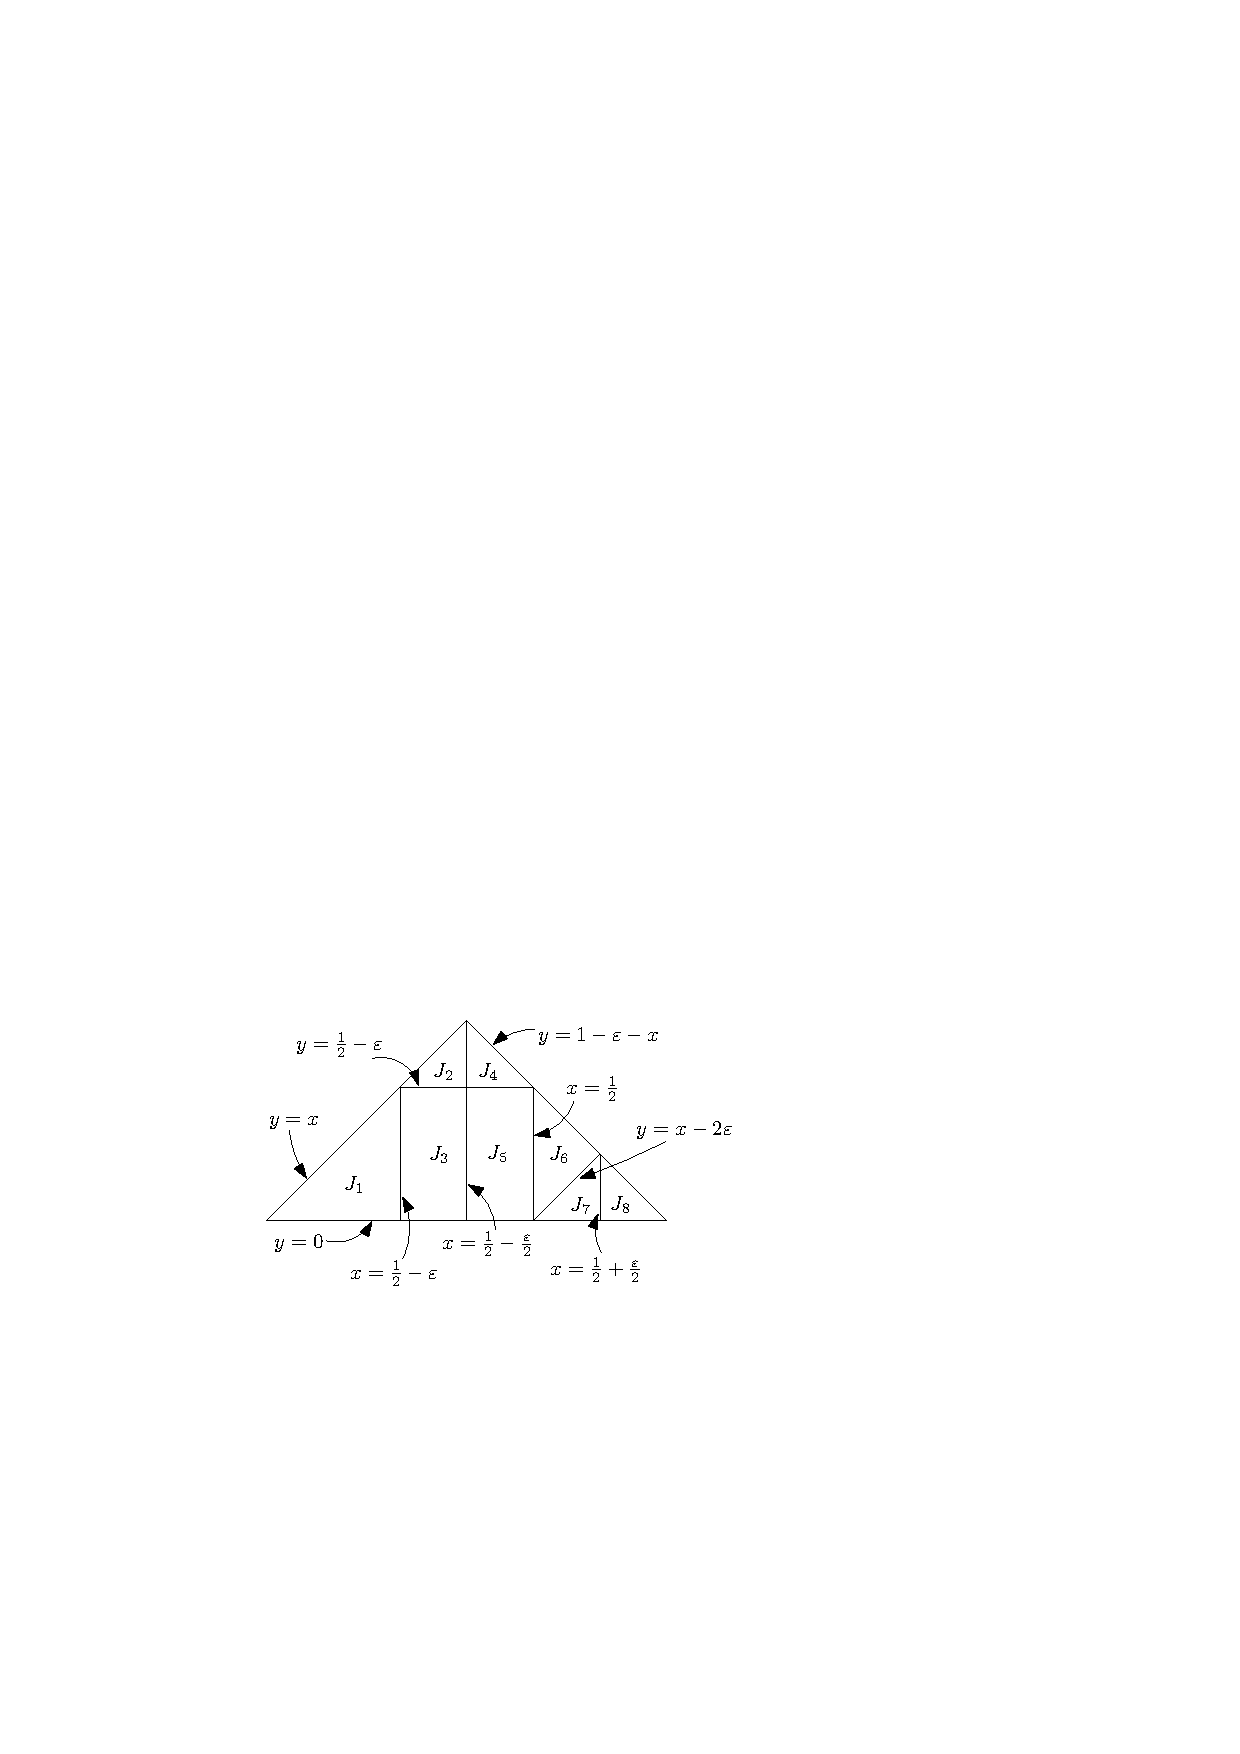
\includegraphics[scale=.5]{xyplot.pdf}\end{center}
The lines in this diagram, moving left to right (and then top to bottom) are $y=x$, $y=0$, $x=1/2-\eps$, $y=1/2-\eps$, $x=1/2-\eps/2$, $x=1/2$, $y=x-2\eps$, and $x=1/2+\eps/2$.  {\bf make sure this picture is drawn to scale when $\eps = 1/4$, and label the regions appropriately.}  We label the pieces of the diagram moving from left to right and then top to bottom, and there are eight corresponding integrals $J_1,J_2,\ldots, J_8$, thus
$$ J = 2( J_1 + \dots + J_8).$$

We have
\begin{align*}
J_1 & =\int_{x=0}^{1/2-\eps}\int_{y=0}^{x} \left(\int_{z=0}^{y}F\downharpoonright_{A_{yzx}}+\int_{z=y}^{x}F\downharpoonright_{A_{zyx}} +\int_{z=x}^{1-\eps-x}F\downharpoonright_{A_{xyz}} +\int_{z=1-\eps-x}^{1-\eps-y}F\downharpoonright_{B_{xyz}}  \right. \\ & \left. +\int_{z=1-\eps-y}^{1+\eps-x}F\downharpoonright_{C_{xyz}} + \int_{z=1+\eps-x}^{1+\eps-y}F\downharpoonright_{U_{xyz}} + \int_{z=1+\eps-y}^{3/2-x-y}F\downharpoonright_{G_{xyz}}\ dz \right)^{2}\ dy\ dx.
\end{align*}
Next comes
\begin{align*}
J_2 & =\int_{x=1/2-\eps}^{1/2-\eps/2}\int_{y=1/2-\eps}^{x} \left(\int_{z=0}^{y}F\downharpoonright_{A_{yzx}}+\int_{z=y}^{x}F\downharpoonright_{A_{zyx}}+\int_{z=x}^{1-\eps-x}F\downharpoonright_{A_{xyz}} +\int_{z=1-\eps-x}^{1-\eps-y}F\downharpoonright_{B_{xyz}}\right. \\ & \left. +\int_{z=1-\eps-y}^{3/2-x-y}F\downharpoonright_{C_{xyz}}\ dz \right)^{2}\ dy\ dx.
\end{align*}
Third is the piece
\begin{align*}
J_3 & =\int_{x=1/2-\eps}^{1/2-\eps/2}\int_{y=0}^{1/2-\eps} \left(\int_{z=0}^{y}F\downharpoonright_{A_{yzx}}+\int_{z=y}^{x}F\downharpoonright_{A_{zyx}} +\int_{z=x}^{1-\eps-x}F\downharpoonright_{A_{xyz}} +\int_{z=1-\eps-x}^{1-\eps-y}F\downharpoonright_{B_{xyz}} \right. \\ & \left. + \int_{z=1-\eps-y}^{1+\eps-x}F\downharpoonright_{C_{xyz}} + \int_{z=1+\eps-x}^{3/2-x-y}F\downharpoonright_{T_{xyz}}\ dz \right)^{2}\ dy\ dx.
\end{align*}

We now have dealt with all integrals involving $A_{xyz}$, and all remaining integrals pass through $B_{zyx}$.  Continuing, we have
\begin{align*}
J_4 & =\int_{x=1/2-\eps/2}^{1/2}\int_{y=1/2-\eps}^{1-\eps-x} \left(\int_{z=0}^{y}F\downharpoonright_{A_{yzx}}+\int_{z=y}^{1-\eps-x}F\downharpoonright_{A_{zyx}} +\int_{z=1-\eps-x}^{x}F\downharpoonright_{B_{zyx}} +\int_{z=x}^{1-\eps-y}F\downharpoonright_{B_{xyz}}\right. \\ & \left. +\int_{z=1-\eps-y}^{3/2-x-y}F\downharpoonright_{C_{xyz}}\ dz \right)^{2}\ dy\ dx.
\end{align*}
Another component is
\begin{align*}
J_5 & = \int_{x=1/2-\eps/2}^{1/2}\int_{y=0}^{1/2-\eps} \left(\int_{z=0}^{y}F\downharpoonright_{A_{yzx}}+\int_{z=y}^{1-\eps-x}F\downharpoonright_{A_{zyx}} \right. \\ & \left. +\int_{z=1-\eps-x}^{x}F\downharpoonright_{B_{zyx}} +\int_{z=x}^{1-\eps-y}F\downharpoonright_{B_{xyz}} +\int_{z=1-\eps-y}^{1+\eps-x}F\downharpoonright_{C_{xyz}} + \int_{z=1+\eps-x}^{3/2-x-y}F\downharpoonright_{T_{xyz}}\ dz \right)^{2}\ dy\ dx.
\end{align*}

The most complicated piece is
\begin{align*}
J_6 & =\left(\int_{x=1/2}^{2\eps} \int_{y=0}^{1-\eps-x} + \int_{x=2\eps}^{1/2+\eps/2}\int_{y=x-2\eps}^{1-\eps-x} \right) \left(\int_{z=0}^{y}F\downharpoonright_{A_{yzx}}+\int_{z=y}^{1-\eps-x}F\downharpoonright_{A_{zyx}} +\int_{z=1-\eps-x}^{x}F\downharpoonright_{B_{zyx}}  \right. \\ & \left. +\int_{z=x}^{1-\eps-y}F\downharpoonright_{B_{xyz}} +\int_{z=1-\eps-y}^{1+\eps-x}F\downharpoonright_{C_{xyz}} + \int_{z=1+\eps-x}^{1/2+\eps}F\downharpoonright_{S_{xyz}}+ \int_{z=1/2+\eps}^{3/2-x-y}F\downharpoonright_{T_{xyz}}\ dz \right)^{2}\ dy\ dx.
\end{align*}
We have now exhausted $C_{xyz}$.  The sixth piece is
\begin{align*}
J_7 & = \int_{x=2\eps}^{1/2+\eps/2}\int_{y=0}^{x-2\eps} \left(\int_{z=0}^{y}F\downharpoonright_{A_{yzx}}+\int_{z=y}^{1-\eps-x}F\downharpoonright_{A_{zyx}} +\int_{z=1-\eps-x}^{x}F\downharpoonright_{B_{zyx}} \right. \\ & \left. +\int_{z=x}^{1+\eps-x}F\downharpoonright_{B_{xyz}} + \int_{z=1+\eps-x}^{1-\eps-y}F\downharpoonright_{E_{xyz}} + \int_{1-\eps-y}^{1/2+\eps}F\downharpoonright_{S_{xyz}}+ \int_{1/2+\eps}^{3/2-x-y}F\downharpoonright_{T_{xyz}} \ dz \right)^{2}\ dy\ dx.
\end{align*}
Finally, we have
\begin{align*}
J_8 & = \int_{x=1/2+\eps/2}^{1-\eps}\int_{y=0}^{1-\eps-x} \left(\int_{z=0}^{y}F\downharpoonright_{A_{yzx}}+\int_{z=y}^{1-\eps-x}F\downharpoonright_{A_{zyx}} +\int_{z=1-\eps-x}^{1+\eps-x}F\downharpoonright_{B_{zyx}} \right. \\ & \left. + \int_{z=1+\eps-x}^{x}F\downharpoonright_{E_{zyx}} + \int_{z=x}^{1-\eps-y}F\downharpoonright_{E_{xyz}} + \int_{1-\eps-y}^{1/2+\eps}F\downharpoonright_{S_{xyz}}+ \int_{1/2+\eps}^{3/2-x-y}F\downharpoonright_{T_{xyz}}\ dz \right)^{2}\ dy\ dx.
\end{align*}

In the case $\eps=1/4$, the marginal conditions \eqref{fmor} reduce to requiring 
\begin{align}
\int_{z=0}^{3/2-x-y}F\downharpoonright_{G_{yzx}}\ dz &= 0\label{m1}\\
\int_{z=0}^{y}F\downharpoonright_{G_{yzx}} +\int_{z=y}^{3/2-x-y}F\downharpoonright_{G_{zyx}}\ dz &= 0\label{m2}\\
\int_{z=0}^{1+\varepsilon-x}F\downharpoonright_{U_{yzx}} + \int_{z=1+\varepsilon-x}^{y}F\downharpoonright_{G_{yzx}} +\int_{z=y}^{3/2-x-y}F\downharpoonright_{G_{zyx}}\ dz &= 0\label{m3}\\
\int_{z=0}^{1+\varepsilon-x}F\downharpoonright_{U_{yzx}} + \int_{z=1+\varepsilon-x}^{3/2-x-y}F\downharpoonright_{G_{yzx}}\ dz &= 0\label{m4}\\
\int_{z=0}^{3/2-x-y}F\downharpoonright_{T_{yzx}}\ dz &= 0\label{m5}\\
\int_{z=0}^{1-\varepsilon-x}F\downharpoonright_{E_{yzx}} + \int_{z=1-\varepsilon-x}^{1-\varepsilon-y}F\downharpoonright_{S_{yzx}} + \int_{z=1-\varepsilon-y}^{3/2-x-y}F\downharpoonright_{H_{yzx}}\ dz &= 0.\label{m7}
\end{align}
Each of these constraints is only required to hold for some portion of the parameter space $\{ (x,y): 1+\eps \leq x+y \leq 3/2 \}$, but as the left-hand sides are all polynomial functions in $x,y$ (using the signed definite integral $\int_b^a = -\int_a^b$), it is equivalent to require that all coefficients of these polynomial functions vanish.

Finally, we take $F(x,y,z)$ to be a polynomial of degree $2$ on each of $A_{xyz},B_{xyz},C_{xyz}$, and use degree $5$ on the other six relevant components of $R$.  More precisely, if we take

\begin{align*}
F\downharpoonright_{A_{xyz}} &:= 1 - \frac{1291x}{1000} + \frac{104x^2}{125} - \frac{659y}{500} + \frac{111xy}{125} + \frac{1099y^2}{1000} - \frac{1257z}{1000} + \frac{637xz}{1000} + \frac{56yz}{125} + \frac{839z^2}{1000} \\
F\downharpoonright_{B_{xyz}} &:= \frac{57}{100} - \frac{303x}{500} + \frac{117x^2}{250} - \frac{136y}{125} + \frac{227xy}{500} + \frac{133y^2}{125} - \frac{303z}{1000} - \frac{9xz}{125} + \frac{57yz}{250} + \frac{37z^2}{250}\\
F\downharpoonright_{C_{xyz}} &:= \frac{17}{50} - \frac{657x}{1000} + \frac{227x^2}{500} - \frac{13y}{20} + \frac{581xy}{1000} + \frac{21y^2}{40} - \frac{9z}{1000} + \frac{3xz}{1000} + \frac{3yz}{200} + \frac{z^2}{250}\\
F\downharpoonright_{E_{xyz}} &:= \frac{4711}{16000} - \frac{199x}{20}00 - \frac{29x^2}{1000} - \frac{2101y}{2000} + \frac{413xy}{1500} + \frac{33y^2}{25} - \frac{19z}{125} - \frac{13xz}{1000} + \frac{31yz}{125} + \frac{7z^2}{600}\\
F\downharpoonright_{S_{xyz}} &:= \frac{2409}{16000} - \frac{9x}{80} - \frac{61x^2}{1000} - \frac{493y}{1000} + \frac{401xy}{1500} + \frac{73y^2}{125} - \frac{73z}{500} + \frac{59xz}{1000} - \frac{9yz}{250} + \frac{7z^2}{1000}\\
F\downharpoonright_{T_{xyz}} &:= -\frac{471}{8000} + \frac{367x}{4000} - \frac{7x^2}{200} - \frac{1133y}{2000} + \frac{9xy}{25} + \frac{129y^2}{200} + \frac{373z}{1000} - \frac{103xz}{400} - \frac{3yz}{200} - \frac{89z^2}{400}\\
F\downharpoonright_{U_{xyz}} &:= -\frac{2548925261}{40960000} + \frac{378889x}{500} - \frac{1486281x^2}{500} + \frac{2109761x^3}{500} - \frac{1806913x^4}{1000} - \frac{823y}{1000} + \frac{1028xy}{125} \\
&\quad - \frac{1276175057x^2y}{20800000} + \frac{5231x^3y}{40} - \frac{604y^2}{125} + \frac{465755881xy^2}{10400000} - \frac{33092919x^2y^2}{400000} + \frac{1941y^3}{500} \\
&\quad - \frac{21127xy^3}{1000} + \frac{28y^4}{125} + \frac{705z}{8} - \frac{196213xz}{200} + \frac{130643581043x^2z}{41600000} - \frac{1270877x^3z}{500} \\
&\quad + \frac{51y^2z}{16000} - \frac{91952143z^2}{3328000} + \frac{619313327xz^2}{2080000} - \frac{18524x^2z^2}{25} + \frac{3y^2z^2}{5000} - \frac{2561z^3}{1000} \\
&\quad + \frac{4869xz^3}{500} - \frac{9z^4}{200}\\
F\downharpoonright_{G_{xyz}} &:= -\frac{2695785741}{10240000} + \frac{2173499391x}{1280000} - \frac{12242903151x^2}{2560000} + \frac{52219413x^3}{10000} - \frac{1806913x^4}{1000} \\
&\quad + \frac{96070478631y}{83200000} + \frac{1007933539xy}{20800000} + \frac{179877147x^2y}{2600000} - \frac{36827397x^3y}{25000} - \frac{669613358991y^2}{166400000} \\
&\quad - \frac{1310180447xy^2}{2600000} + \frac{10110876x^2y^2}{3125} + \frac{19620542273y^3}{3900000} - \frac{17662711xy^3}{12500} - \frac{1806913y^4}{1000} \\
&\quad + \frac{104838525951z}{166400000} - \frac{126851653541xz}{41600000} + \frac{15524384001x^2z}{2600000} - \frac{20898059x^3z}{6250} - \frac{1531159429yz}{640000} \\
&\quad + \frac{14385788557y^2z}{2600000} - \frac{20898059y^3z}{6250} - \frac{91851736253z^2}{166400000} + \frac{4642413047xz^2}{2600000} - \frac{738812349x^2z^2}{400000} \\
&\quad + \frac{2655529yz^2}{1625} - \frac{756836049y^2z^2}{400000} + \frac{1081347403z^3}{5200000} - \frac{33823447xz^3}{100000} - \frac{36827397yz^3}{100000} \\
&\quad - \frac{2238403z^4}{80000}\\
F\downharpoonright_{H_{xyz}} &:= -\frac{37{250}} + \frac{71x}{500} - \frac{109x^2}{1000} + \frac{6z}{125} - \frac{3xz}{1000} - \frac{9z^2}{250}
\end{align*}

then one can compute that $I(F) = 0.03057904694\dots$ and $J(F) = 0.06116827145\dots$, with all the marginal conditions \eqref{m1}-\eqref{m7} obeyed, giving the claim.
